\documentclass[12pt]{article}

\usepackage[margin=0.8 in]{geometry}
\usepackage{amsmath}
\usepackage{amssymb}
%\usepackage{macros}
\usepackage{mathtools}
\usepackage{enumerate}
\usepackage{verbatim}
\usepackage{amsthm}
\usepackage{hyperref}

\title{}
%\content{}



\let \proj \undefined
\newcommand{\tr}{ \mathrm{tr}}
\DeclareMathOperator{\SU}{SU}
\DeclareMathOperator{\proj}{proj}
\newcommand{\sS}{\mathscr{S}}
\DeclareMathOperator{\comp}{comp}
\newcommand{\A}{\mathcal{A}}
\newcommand{\D}{\mathcal{D}}
\newcommand{\e}{\epsilon}
\newcommand{\Are}{\A_{r,\e}}
\newcommand{\Kre}{K_{r,\e}}
\newcommand{\Dre}{\D_{r,\e}}
\newcommand{\rt}{\tilde{r}}
\newcommand{\et}{\tilde{\e}}
\newtheorem{definition}{Definition}
\newenvironment{solution}
  {\begin{proof}[Solution]}
  {\end{proof}}
\newtheorem{example}{Example}
\newtheorem{exercise}{Exercise}

\newcommand{\vr}{\vec{r}}
\newcommand{\vF}{\vec{F}}
\newcommand{\R}{\mathbb{R}}


\begin{document}
\section*{Line integrals}
What to know:
\begin{enumerate}
\item Be able to parametrize curves
\item Be able to set up and compute line integrals with respect to arc length $(ds)$ and of vector fields ($\cdot d\vr$).
\item Be able to compute line integrals $dx$ and $dy$ (interpreted as special cases of integrals of vector fields).
\item Know which line integrals depend on the parametrization of the curve and which ones don't.
\end{enumerate}




In this section, we'll see how to integrate over curves. The curves we'll talk about are called piecewise smooth curves, which means that they are finite unions of smooth curves, parametrized as $c(t)=(x(t),y(t))$, $t\in [a,b]$, like in figures \ref{fig3} and \ref{fig4}\footnote{The precise definition of a piecewise smooth curve is that you want the derivative $\dot{c}(t)=(\dot{x}(t),\dot{y}(t))$ to exist and be continuous for all except maybe finitely many $t\in [a,b]$, and the side limits $\lim_{t\to t_0^\pm }\dot{x}(t)$ to exist for all $t_0\in[a,b]$. This is to exclude some pathological but quite exciting cases, like the one in figures \ref{fig1} and \ref{fig2}, or even space filling curves!} . 


\begin{figure}[h]
\centering
\parbox{5cm}{
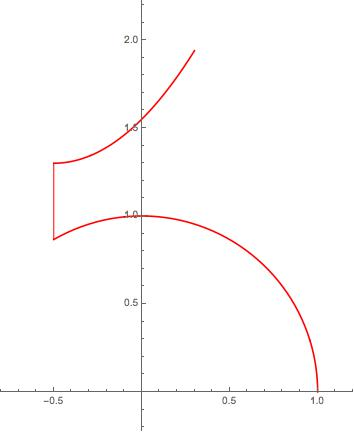
\includegraphics[width=5cm]{pwsm.jpeg}
\caption{A piecewise smooth curve}
\label{fig3}}
\qquad
\begin{minipage}{5cm}
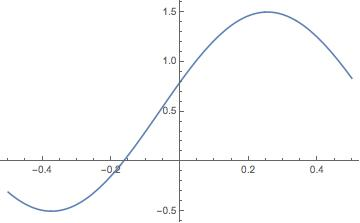
\includegraphics[width=5cm]{pwsm2.jpeg}
\caption{Another piecewise smooth curve}
\label{fig4}
\end{minipage}
\end{figure}



\begin{figure}[h]
\centering
\parbox{5cm}{
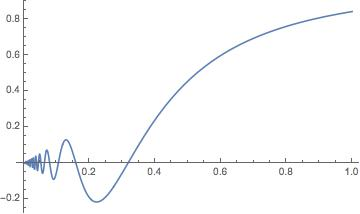
\includegraphics[width=5cm]{topologist.jpeg}
\caption{The graph of $f(x)=x\sin(1/x)$, not piecewise smooth}
\label{fig1}}
\qquad
\begin{minipage}{5cm}
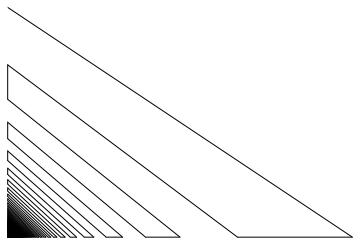
\includegraphics[width=5cm]{zig.jpeg}
\caption{A curve consisting of infinitely many line segments, not piecewise smooth}
\label{fig2}
\end{minipage}
\end{figure}


\subsection*{Line integrals of scalar functions}
 Suppose that $f(x,y)$ is a continuous non-negative function. Our goal is to be able to evaluate the area of a fence that lies above the curve $c$ and under the graph of $f$. 




To do this, we approximate the area in the following way: We first approximate the curve $c$ by line segments $[a_j,a_{j+1}]$ and form rectangles (living in $\R^3$) with base $[a_j,a_{j+1}]$ and height $f(a_j^*)$, where $a_j^*$ is the midpoint of each line segment. Then, we evaluate the area of each of those rectangles and sum the areas. As we make the approximation of the curve more and more accurate, this procedure gives rise to a special type of integral, called \textbf{line integral with respect to to arc length.}

(you can find an animated graph of this procedure \href{http://sites.math.washington.edu/~neptamin/324Au17/Mathematica/}{here}).

\begin{definition}
The line integral with respect to arc length of a continuous function $f(x,y)$ along a piecewise smooth curve $c(t)=(x(t),y(t))$, $a\leq t \leq b$, is defined to be $$\int_c f(x,y)ds=\int_a^b f(x(t),y(t))\sqrt{\left(\frac{d x}{dt}\right)^2+\left(\frac{d y}{dt}\right )^2}dt.$$
\end {definition}
Remarks: \begin{itemize}
\item Note that if we replace $f$ by the function 1 we obtain the length of $c$!
\item Another physical interpretation of a line integral with respect to arc length is that when you have the density function $\rho$ of a wire lying on a plane curve $c$, its mass is given by $$m=\int_c\rho(x,y)ds.$$
\end{itemize}
\begin{example} Find $\int_c x ds$, where $c$ is the right half of a circle with radius 2.
\end{example}
\begin{solution}
We first parametrize $c$: a way to do it is by choosing $c(t)=(2\cos(t),2\sin(t))$, $-\pi/2\leq t\leq \pi/2$. Then, compute $x'(t)=-2\sin(t)$, $y'(t)=2\cos(t)$ and write $$\int_c x ds=\int_{-\pi/2}^{\pi/2}(2\cos(t))\sqrt{4\sin^2(t)+4\cos^2(t)}dt=8$$
\end{solution}

Wait! How do we know that this is the correct way to parametrize this curve? We know that there are many different ways this can be done. Does it matter how fast we go or in which direction?

\begin{exercise} Now parametrize the curve of the last example using $c(t)=(2 \cos(-2t),2\sin(-2t))$, for $-\pi/4\leq t\leq \pi/4$ (this follows the same path, but twice as fast and in opposite direction). What do you find? 
\end{exercise}

In fact, line integrals with respect to arc length \textbf{do not depend on the parametrization}, as long as the curve is only transversed once: (for example, a case where you would find different answers is if you try to parametrize the unit circle by $c_1(t)=(\cos(t),\sin(t))$, $0\leq t\leq 2\pi $ and $c_2(t)=(\cos(t),\sin(t))$, $0\leq t\leq 3\pi $). This makes the question asked in Example 1 a valid one: no matter which way we choose to parametrize the curve, we'll find the same answer.

Now that we know that the parametrization doesn't matter as long as we have one, let's remember a few ways to actually find it if necessary.



The definition of the line integral with respect to arc length for a function $f(x,y,z)$ is completely analogous:
\begin{definition}
The line integral with respect to arc length of a continuous function $f(x,y,z)$ along a piecewise smooth curve $c(t)=(x(t),y(t),z(t))$, $a\leq t \leq b$, is defined to be $$\int_c f(x,y,z)ds=\int_a^b f(x(t),y(t),z(t))\sqrt{\left(\frac{d x}{dt}\right)^2+\left (\frac{d y}{dt}\right )^2+\left (\frac{d z}{dt}\right )^2}dt.$$
\end {definition}

The parametrization of some standard curves can be found  \href{http://sites.math.washington.edu/~neptamin/324Au17/Notes/Handout1/handout1.pdf}{here}.


\section*{Line Integrals of Vector Fields}
So far, we've seen how we can integrate scalar functions. Now we want to make sense of integration of vector fields along curves, and the motivation comes from physics: In physics, we are interested in knowing the work produced by a force field when an object moves along a curve $c$ given by the vector function $\vr(t),$ $t\in[a,b]$ inside the force field $\vF (x,y)$. 

We know from physics that the work produced by a constant force $\vec{G}$ while an object is displaced by $\vec{x}$ is given by $\vec{x}\cdot\vec{G}$. In our case, we have a variable force (a force field) $\vF$ and a variable direction of movement. So, when trying to make sense of the total work produced by $\vF$ on an object moving along $c$, the natural thing to do is to split the curve into very short curves, where the displacement is happening in an almost constant direction ($\vr\hspace{1 mm}'(t)$!) and the  force is also almost constant and equal to $\vF(\vr(t))$. Then the infinitesimal work produced by $\vF$ for time $t$ would be $$\vF(\vr(t))\cdot\vr\hspace{1 mm}'(t).$$
We'd finally sum these infinitesimal quantities, that is, integrate!

We have:
\begin{definition}
Let $\vF(x,y)$ be a continuous vector field and $c(t)=\vr(t), t\in[a,b]$ be a curve in $\R^2$. We define the line integral of $\vF$ along $c$ to be $$\int_c\vF\cdot d\vr=\int_a^b\vF(\vr(t))\cdot \vr\hspace{1 mm}'(t)dt.$$
\end{definition}
\begin{example}
Compute $\int_c\vF\cdot d\vr$, where $\vF(x,y)=\langle x^2,-xy\rangle$ and $c$ is the line segment from (1,0) to (0,1) parametrized by $c(t)=\vr(t)=(1-t,t)$, $t\in [0,1]$.
\end{example}
\begin{solution} We have $\vr\hspace{1 mm}'(t)=\langle -1,1\rangle$, so $$\int_c\vF\cdot d\vr=\int_0^1-(1-t)^2-t(1-t)dt=-1/2.$$
\end{solution}
\begin{exercise}
Now try to parametrize the segment in the above example differently: Use $c(t)=\vr(t)=(2t,1-2t),$ $t\in[0,1/2]$ (this travels along the segment in double speed and opposite direction).
\end{exercise}
In the last exercise, you should find the answer to be $1/2$. You may have noticed that the sign is different from the one we found in the solution before. However, nothing else seems to have changed. This is not an accident. The line integrals of vector fields do not depend on the speed of the parametrization, but \textbf{they do depend on the direction that the curve is transversed}. This means that if a problem asks to compute such an integral, it must provide a parametrization, or at least direction in which the curve is transversed.

If $c$ is a curve, let us denote by $-c$ a curve that consists of the same set of points as $c$, but is transversed in the opposite direction (regardless of the speed). Then \begin{equation}\label{eq1}\int_{-c}\vF\cdot d\vr=-\int_c \vF\cdot d\vr.\end{equation}

So, if we are trying to solve a problem that that asks to compute a line integral of a vector field along a curve and only gives us the direction in which a curve is transversed but not an exact parametrization, here's what we can do: We find a parametrization and check if our parametrization agrees with the direction given in the problem: if it does, we're fine; if not, we integrate with the parametrization we found and then use \eqref{eq1} to say that the final answer has the opposite sign of the one we found.

Now, by unwinding the definition, if $c(t)=\vr(t)=(x(t),y(t))$, $t\in[a,b]$ and $\vF(x,y)=\langle P(x,y), Q(x,y)\rangle$, \begin{equation}\label{eq2}\int_{c}\vF\cdot d\vr=\int_a^b P(x(t),y(t))x'(t)+Q(x(t),y(t))y'(t)dt.\end{equation}

\textbf{Notation}: we write \begin{equation}\label{eq3}\int_a^b P(x(t),y(t))x'(t)dt=:\int_cP(x,y)dx\end{equation} and similarly \begin{equation}\label{eq4}\int_a^b Q(x(t),y(t))y'(t)dt=:\int_cQ(x,y)dy.\end{equation} So, \eqref{eq2} can be written as \begin{equation}\label{eq5}\int_{c}\vF\cdot d\vr=\int_cP(x,y)dx+\int_c Q(x,y)dy.\end{equation} You will often see this last notation abbreviated as $$\int_cP(x,y)dx+\int_c Q(x,y)dy=:\int_cP(x,y)dx+ Q(x,y)dy.$$
Remark: Many textbooks (including Stewart's) define the right hand sides of \eqref{eq3} and \eqref{eq4} as two more types of line integrals of scalar functions, besides the line integral with respect to arc length and deduce \eqref{eq5} as a consequence. In our setting, we can interpret $\int_cf(x,y)dx$ as the line integral of the vector field $\vF(x,y)=\langle f(x,y), 0\rangle $ along $c$, and similarly for $\int_cf(x,y)dy$. To compute them, \eqref{eq3} and \eqref{eq4} give $$\int_cf(x,y)dx=\int_a^bf(x(t),y(t))x'(t)dt$$ and similarly for $\int_cf(x,y)dy$.


 The definitions and properties related to line integrals of vector fields carry over unchanged when we have vector fields in $\R^3$ and curves in $\R^3$: Just include a variable $z$! We have
\begin{definition}
Let $\vF(x,y,z)$ be a continuous vector field and $c(t)=\vr(t)=\langle x(t),y(t),z(t)\rangle$, $t\in[a,b]$ be a piecewise smooth curve in $\R^3$. We define the line integral of $\vF$ along $c$ to be $$\int_c\vF\cdot d\vr=\int_a^b\vF(\vr(t))\cdot \vr\hspace{1 mm}'(t)dt.$$
\end{definition}

\end{document}

